\chapter{Layout
\index{Chapter!Layout}
\index{Layout}
\label{Layout}}
\section{Intro to PCBs}
Before getting into the meat and potatoes of how to design a PCB, I think it is worthwhile to go over the terms and basics surrounding PCBs.
When starting this project I didn't know anything, and probably still don't, however it helps to know the terms and have context when
watching tutorials and reading documentation, etc.

\subsection{PCB Layers}

\begin{figure}[H]
  \centering
  \scalebox{.7}{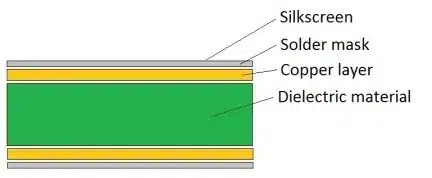
\includegraphics{AllegroImages/layersOverview.jpg}}
\caption{PCB Layers}
\label{img:pcblayers}
\end{figure}

A Printed Circuit Board (PCB) is made up of different materials all stacked up on top each of other, where each of these materials is called
a layer of the PCB. You will also hear the term "stackup" used to describe the amount and kind of layers in one PCB. There are essentially
only four types of layers you need to know, as shown in Figure \ref{img:pcblayers}. The first and most important one is the copper layer.
Copper is a conductor, and so this is the layer in which we place copper where we want to conduct electricity. Whether its for sending power or
signals from one place to another, or placing copper where we want to solder our component pads, this is the place where the actual circuitry is outlined.
You can notice however there are two copper layers in Figure \ref{img:pcblayers}, both of which can have different signals passing through them.
In order to separate the two conductors to prevent shorts, we use a substrate layer, also referred to as a dielectric material. The dielectric
layer goes between copper layers, with one purpose being electrical insulation to keep copper layers from shorting or inducing current in
one another. While it does not conduct electricity, it has a controlled impedance meaning signals won't have weird reactions in different
parts of the board and behavior of signals can be predicted. Different dielectric materials have different dielectric constants, essentially
the number you can use to determine the constant impedance across the board. Now that we have a dielectric and copper layer, we can place a bunch
of copper layers separated by dielectric layers to fit a lot of circuitry in a small space. The third layer we need is the soldermask. The top
and bottom copper layers are exposed to the elements, while all copper layers in the middle are safe within the board. These top and bottom layers
have exposed copper that are subject to things like oxidation, solder shorts between copper areas, and reduces affect of things like moisture.
So, the soldermask is simply a film that goes on top of the top and bottom copper layers to protect it. Finally, the silkscreen layer is just
engraved writing on the soldermask to help humans when assembling the components onto the board. 

\section{Traces and Vias}
\begin{figure}[H]
  \centering
  \scalebox{.7}{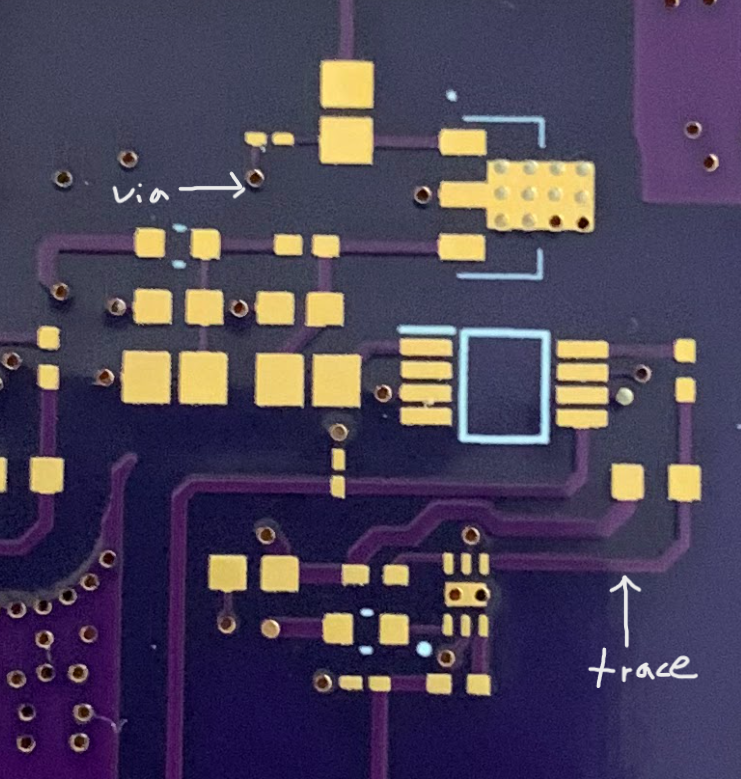
\includegraphics{AllegroImages/tracesandvias.png}}
\caption{Traces and Vias from Mithril Board}
\label{img:tracesandvias}
\end{figure}

In the last section, we mentioned copper layers being where copper is layed down where we want to transmit electricity from one place
to another. This means we have to connect different components, power sources, grounds, etc. with strips of copper which we call traces. As 
can be seen in Figure \ref{img:tracesandvias}, traces can vary in width, orientation, etc., and are basically drawn out by the designer based
on where they want their electricity to go. Their width, orientation, etc. are important, and their affects can be found in Chapter \ref{Radar Theory}.
We also discussed that there can be multiple layers of copper within a board which is great for saving space, but how can we connect one layer
of copper to another when there is an insulated dielectric between them? The answer is vias, which are copper plated holes drilled in the board
that allow for connection of copper in different layers. As can be seen in Figure \ref{img:tracesandvias}, the vias are very small holes which
can vary in diameter and connect to a trace. Like traces, the via diameter can affect its conductive properties in a similar fashion. By using
traces and vias in tandem, we can build out our schematic in a small, consolidated board.

\section{Components}
\begin{figure}[H]
  \centering
  \scalebox{.4}{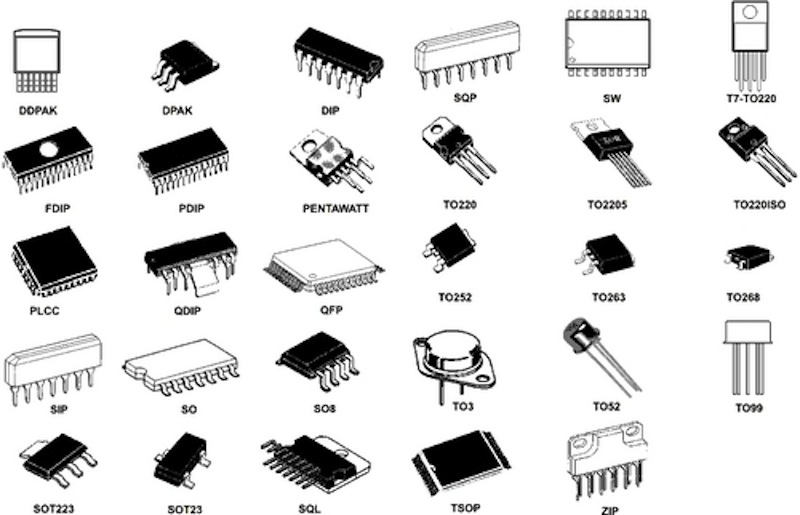
\includegraphics{AllegroImages/componentTypes.jpg}}
\caption{Component Package Types}
\label{img:componentpackage}
\end{figure}
Traces and vias are only useful when they are used with components that execute some task. Whether it be primitive parts like resistors and capacitors
or integrated circuits, components are what make a PCB functional. Components usually come in standardized shapes with standardized pin placements
called packages. Some common package types can be found in Figure \ref{img:componentpackage}. These components will eventually be soldered
onto the PCB, so the designer must put solder pads for the component pins with correct spacing, pitch (width), and orientation. 

\begin{figure}[H]
  \centering
  \scalebox{.4}{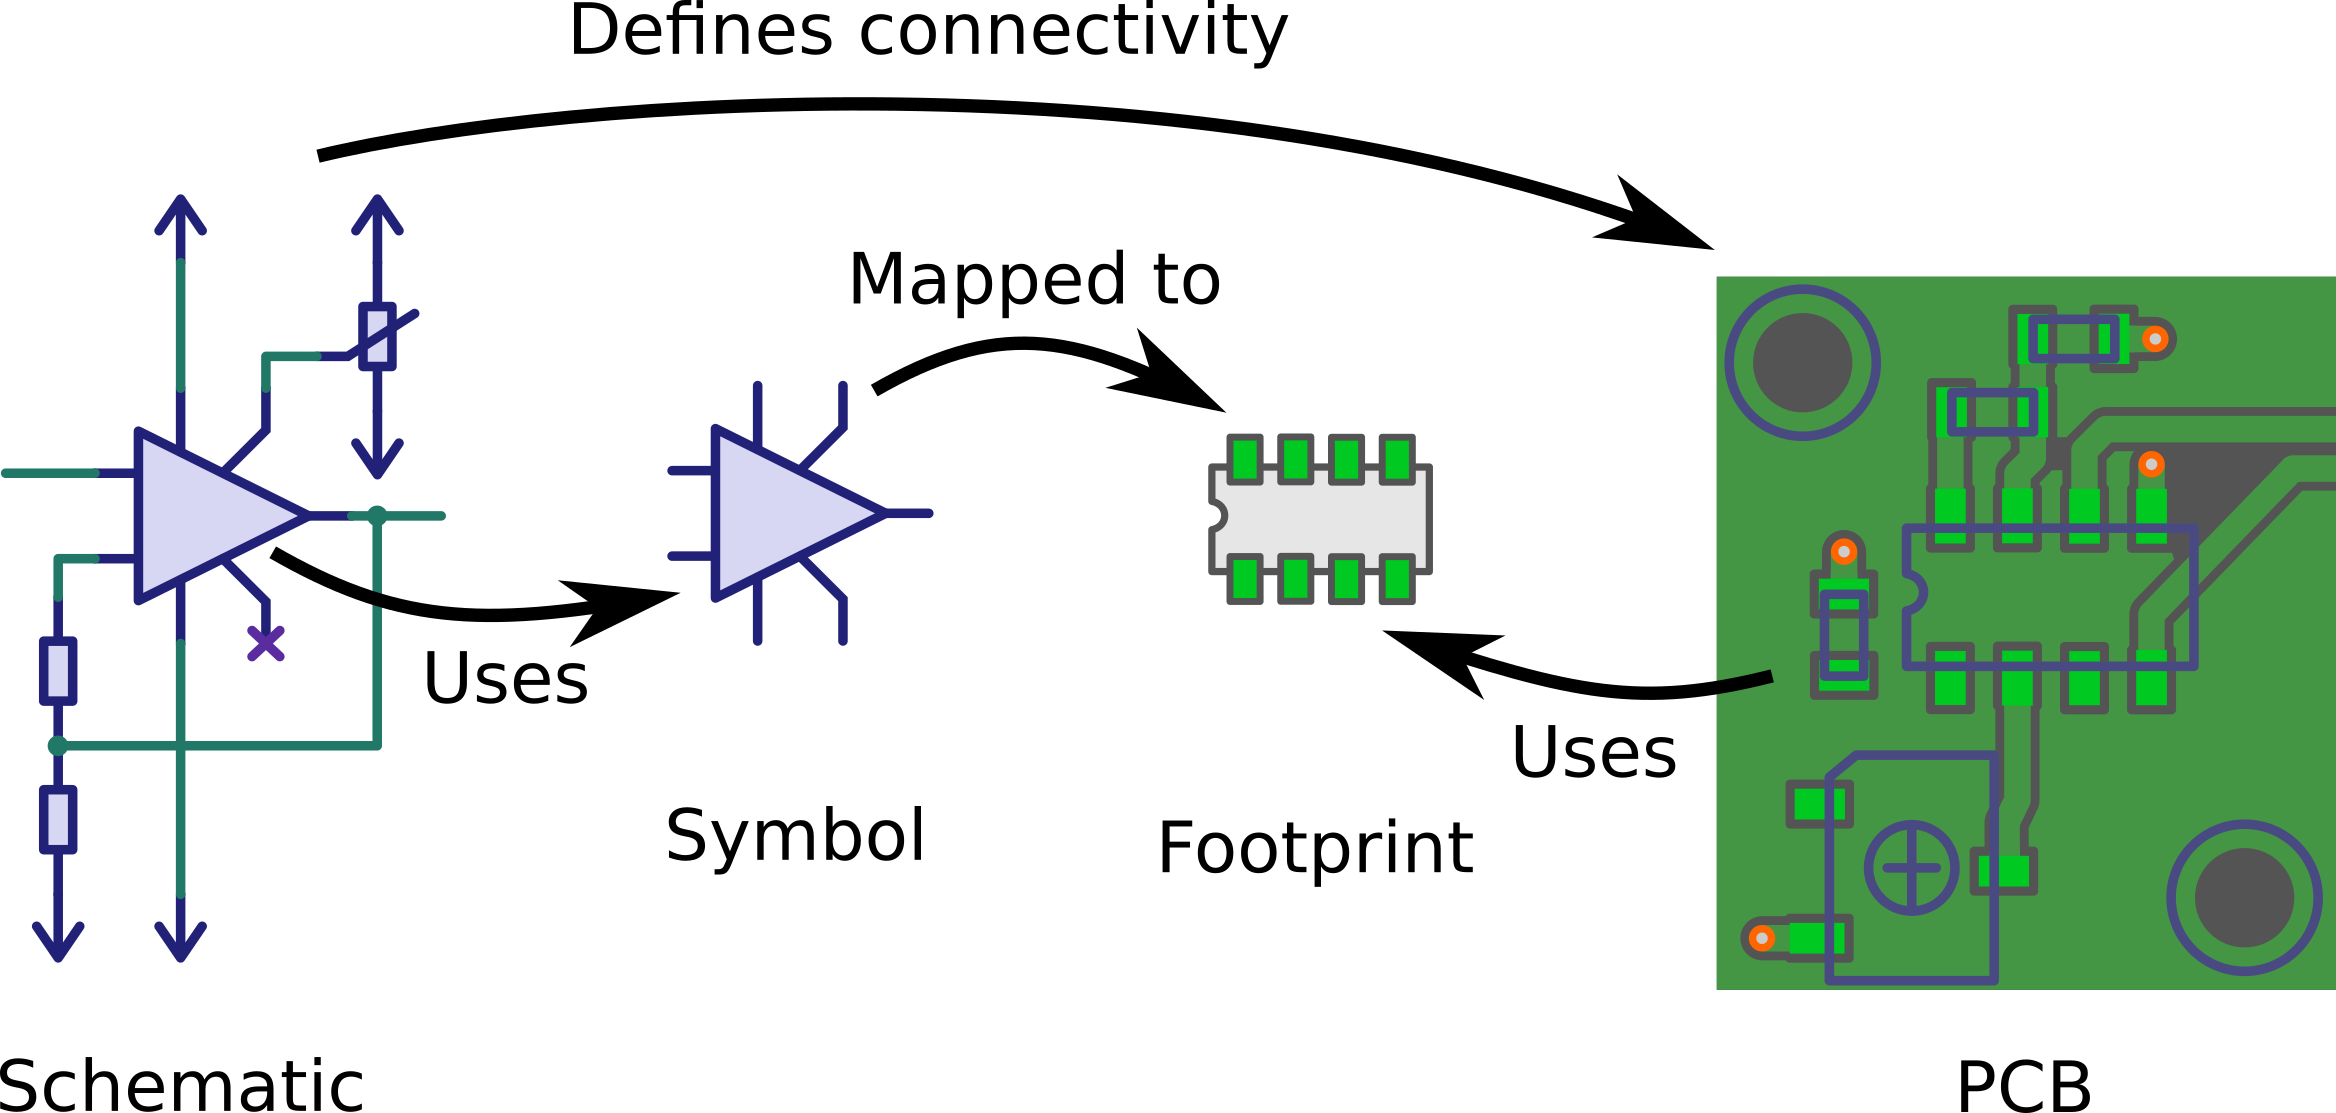
\includegraphics{AllegroImages/footprint.png}}
\caption{Footprint Schematic Symbol Relationship}
\label{img:footprint}
\end{figure}

Instead of the designer drawing all the solder pads with exactly the right dimensions by hand, CAD tools help in creating a "footprint" or a
digital drawing of the size and solder pads of a component. Footprints encapsulate all the physical aspects of a component as mentioned above,
and the designer can map the schematic symbol pins of the same part to the footprint so they know what connects where as can be seen in Figure \ref{img:footprint}.
These footprints follow physical dimensions found in a component's datasheet, and most parts have a footprint out there that someone else made which
you can essentially drag and drop into your design.

\section{Printing and Assembling}
Once you have created your PCB with layers, traces, vias, and components, its time to print the board, order the parts, and assemble the board.
The main deliverables when printing and assembling a board are "Gerbers", a Bill of Materials(BOM), and drill files. Gerbers are ASCII standardized
files that describe all the parts of your PCB (coordinates of parts, orientation of traces, traces on different layers, etc) and are what
printers use to automate the printing process. CAD tools generate these files after your PCB is done, and you can simply send these to your
manufacturer to get your board printed! The BOM describes all the components that are used in your design and makes it easy for you to source
your parts. Drill files specify the locations of vias and chassis treads or any other holes you might have in your board, and again are generated
by your CAD tool.

\section{Allegro Overview}
\begin{figure}[H]
  \centering
  \scalebox{.4}{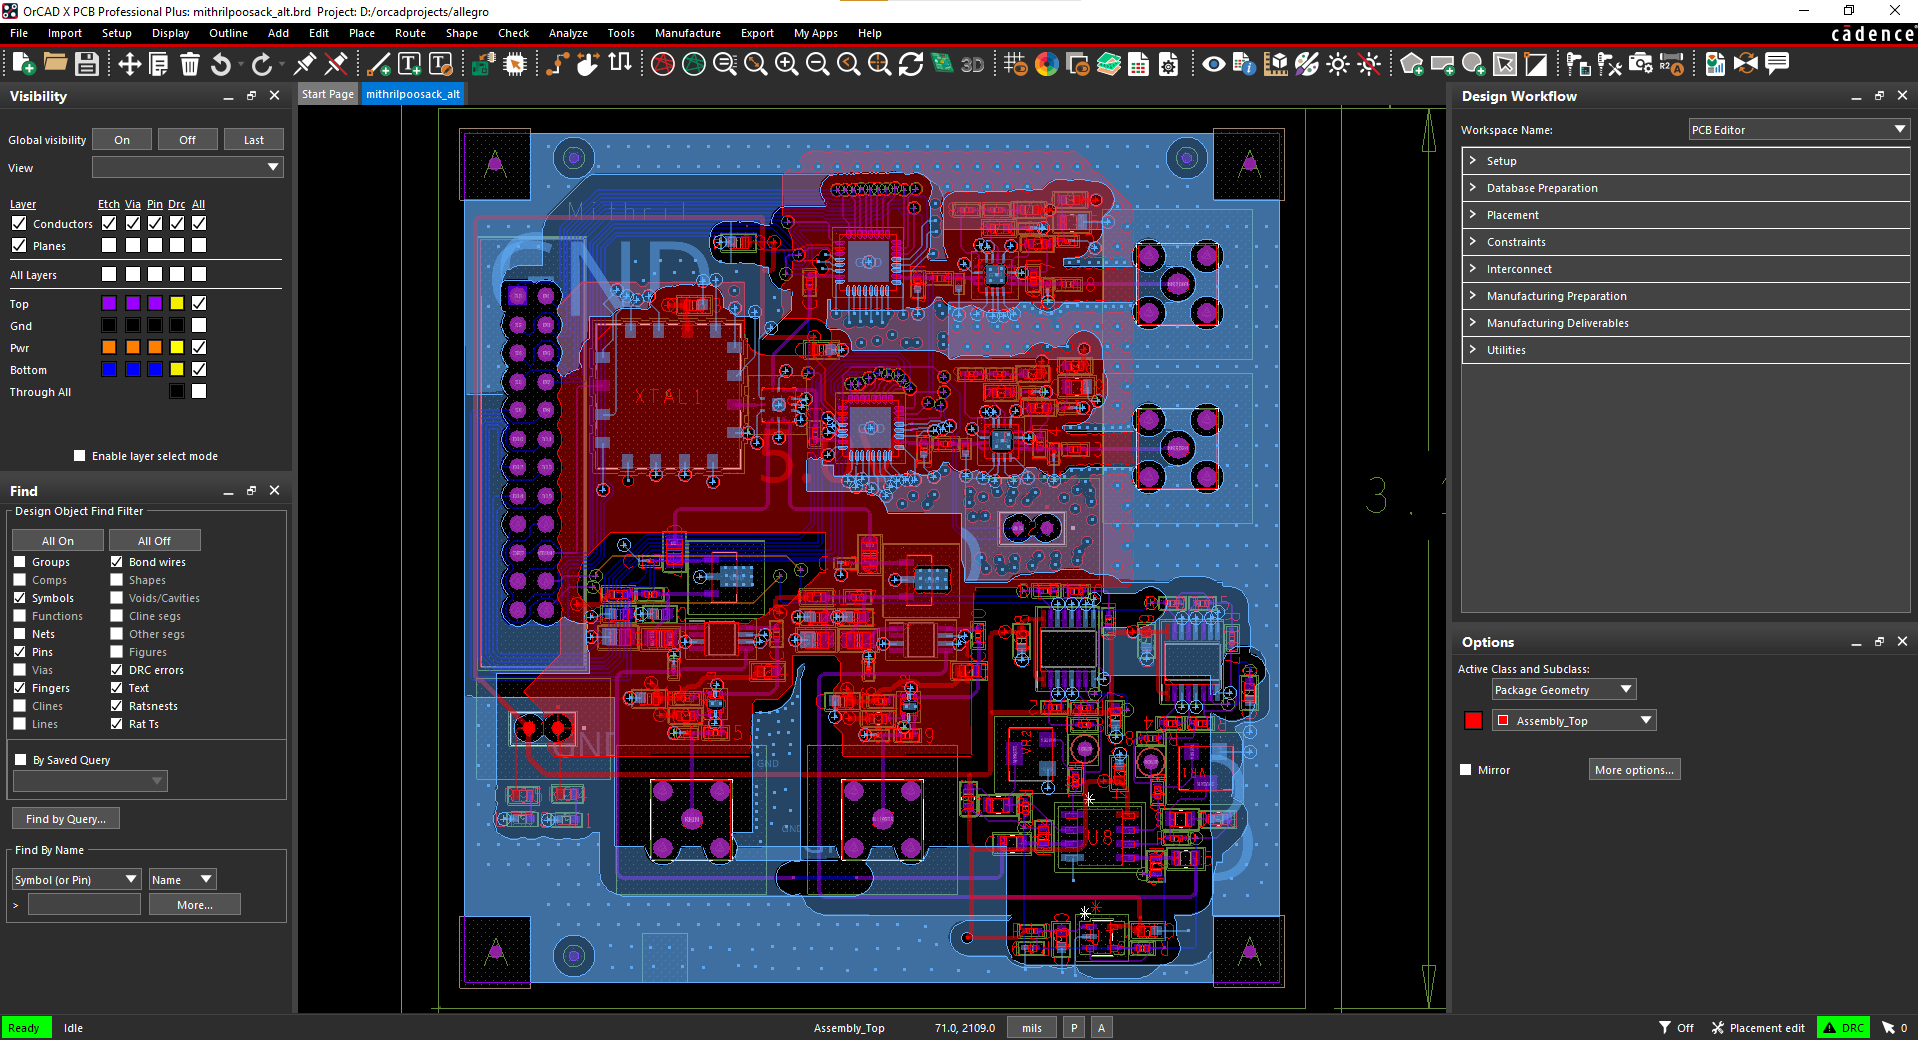
\includegraphics{AllegroImages/layoutfull.png}}
\caption{Allegro Layout}
\label{img:layoutfull}
\end{figure}

First we went over how to create a schematic in Capture CIS, now we will go over Allegro. Allegro is
Cadence's counterpart to Capture which allows you to design a layout for the schematic that can be
printed and assembled to create a functioning printed circuit board.

\begin{figure}[H]
  \centering
  \scalebox{.7}{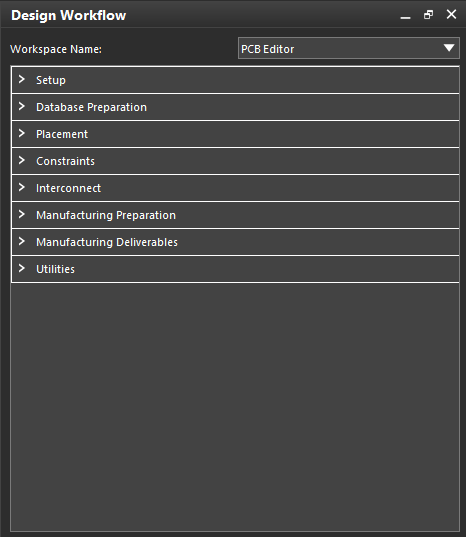
\includegraphics{AllegroImages/designworkflow.png}}
\caption{Design Workflow}
\label{img:designworkflow}
\end{figure}

The most important feature in Allegro is the design workflow. This pane shows all the steps you need to take in order to design a PCB
in Allegro. We will go through all of these panes in the following sections, but make sure to have it open in your Allegro window to quickly
go back and forth from different editing modes.

\begin{figure}[H]
  \centering
  \scalebox{.7}{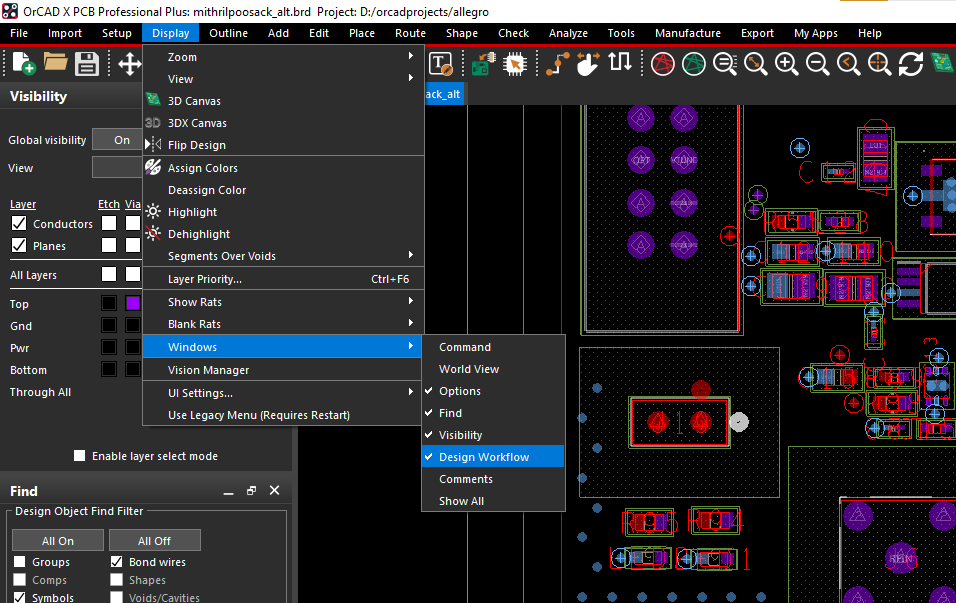
\includegraphics{AllegroImages/windowsTab.png}}
\caption{How to Display Design Workflow}
\label{img:workflowTab}
\end{figure}

If you do not see the design workflow pane in your design, on the top bar navigate to Display, Windows, and then select Design Workflow. You can then drag
and drop the pane to put it wherever you want.

\subsection{Design Setup}

\begin{figure}[H]
  \centering
  \scalebox{.7}{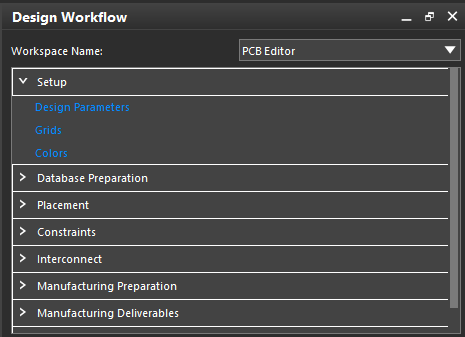
\includegraphics{AllegroImages/setupPane.png}}
\caption{Design Setup}
\label{img:setupPane}
\end{figure}

For Mithril, we followed the design workflow almost verbatim, and this is the workflow we will describe in this tutorial. The first step
is setting up the design to fit our specifications. You can find the setup pane as shown in Figure \ref{img:setupPane}.

\begin{figure}[H]
  \centering
  \scalebox{.7}{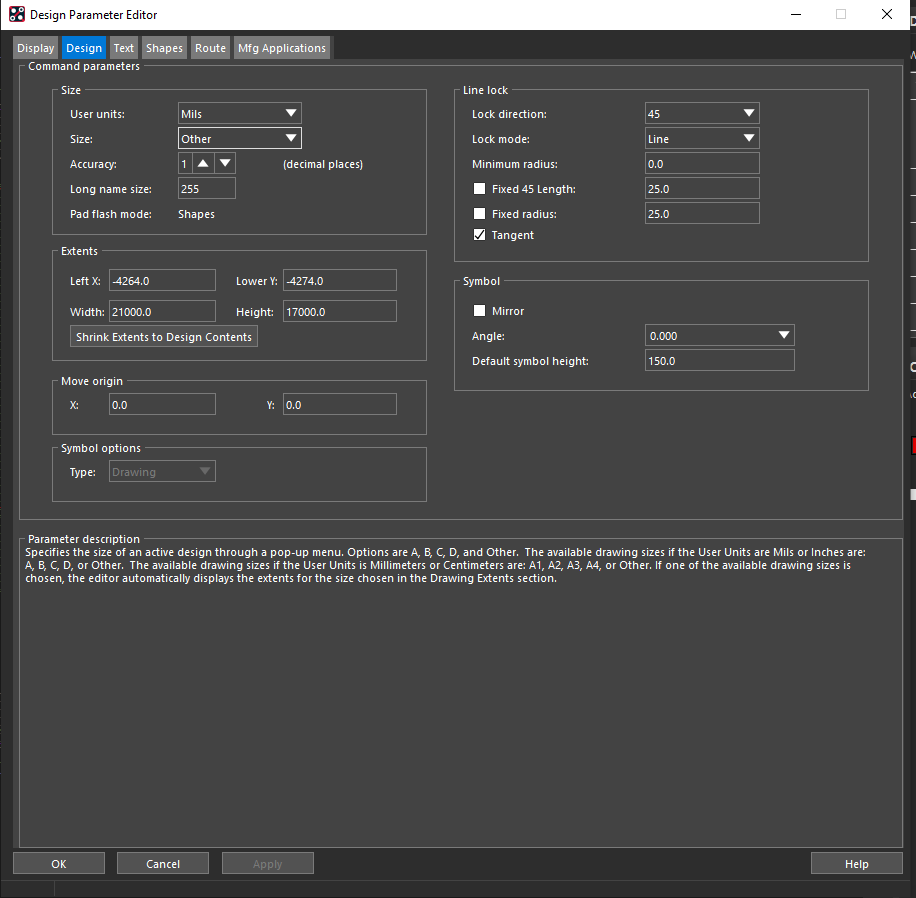
\includegraphics{AllegroImages/designTabSetupPane.png}}
\caption{Design Tab}
\label{img:designTabSetupPane}
\end{figure}

After clicking on "Design Parameters", you can navigate to the Design tab as seen in Figure \ref{img:designTabSetupPane}. Honestly,
this is the only tab that has stuff you want to change. One important thing to change is the user units, which is normally mils (tenth of inch)
or millimeters. You can also switch grids on here, but I prefer them off to be honest.

\begin{figure}[H]
  \centering
  \scalebox{.6}{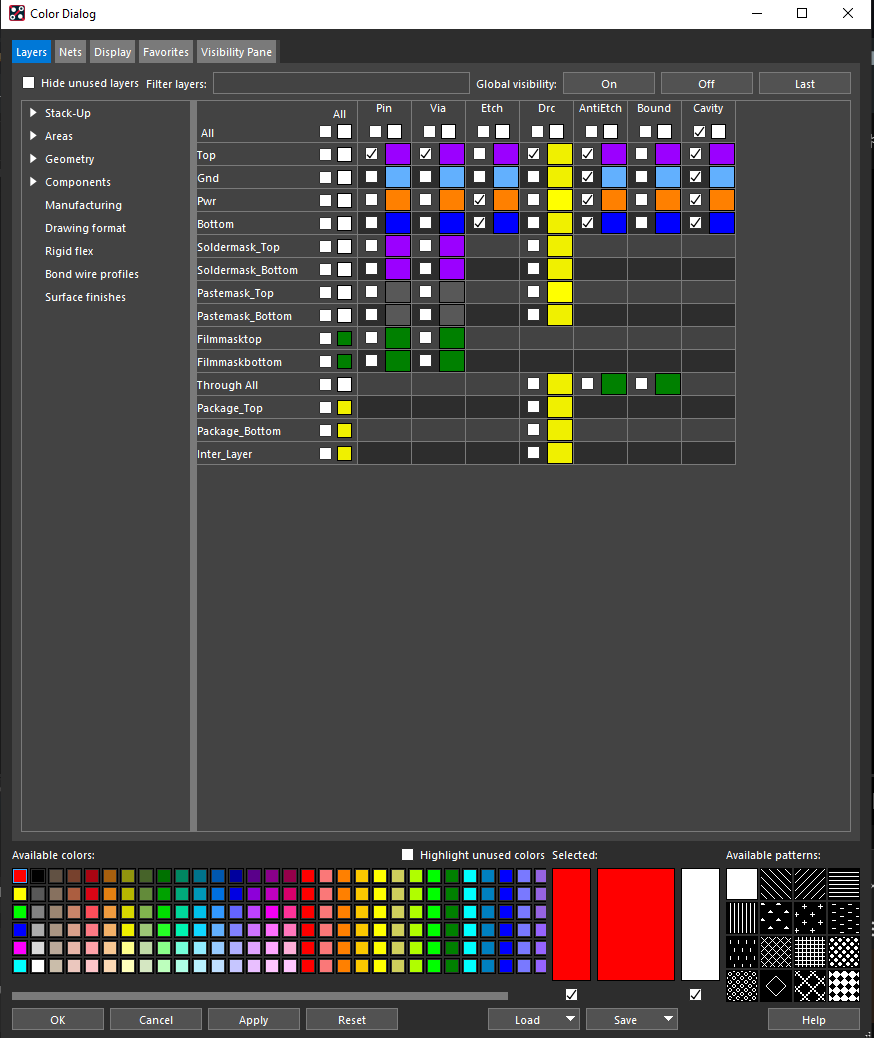
\includegraphics{AllegroImages/colorsTabSetupPane.png}}
\caption{Layer Colors}
\label{img:colorsTabSetupPane}
\end{figure}

The next, and quite frankly a very important tool, is the color tab. This is all really preference, but the defaults in Allegro are pretty bad
and make it hard to see when designing. In the "Layers" tab, there are several drop downs of types of objects that you can set colors for.
You can see my Stack-Up section preferences in Figure \ref{img:colorsTabSetupPane}, and to change colors you click a color on the bottom of the dialog,
then click the little boxes next to a layer and type of object above it. The structure I used was to make everything in a layer the same color except DRC (Design Rule Check)
which points out if you have an error. The first four rows are for my four layers, so I made sure to make them distinct colors. 

\begin{figure}[H]
  \centering
  \scalebox{.6}{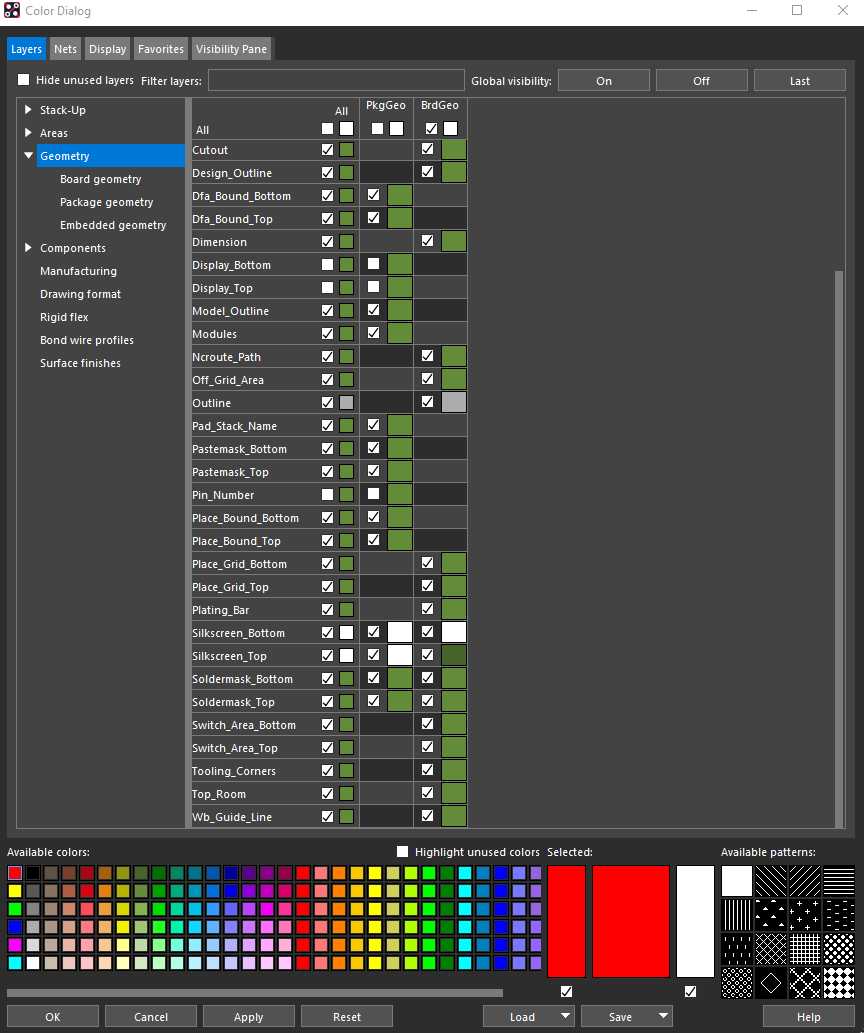
\includegraphics{AllegroImages/colorsGeometry.png}}
\caption{Geometry Colors}
\label{img:geometryColors}
\end{figure}

The layers will make it much easier to distinguish between layers, but there is a lot of bloat text that comes up on the screen with 
Allegro defaults. So, in the "Geometry" tab of the colors dialog I switched off "DisplayBottom", "DisplayTop", and "PinNumber". I also changed
the silkscreen text to white to make it easier to see. This will help with visibility in the long run, and you can see what the geometry
dialog looks like in \ref{img:geometryColors}.

\begin{figure}[H]
  \centering
  \scalebox{.6}{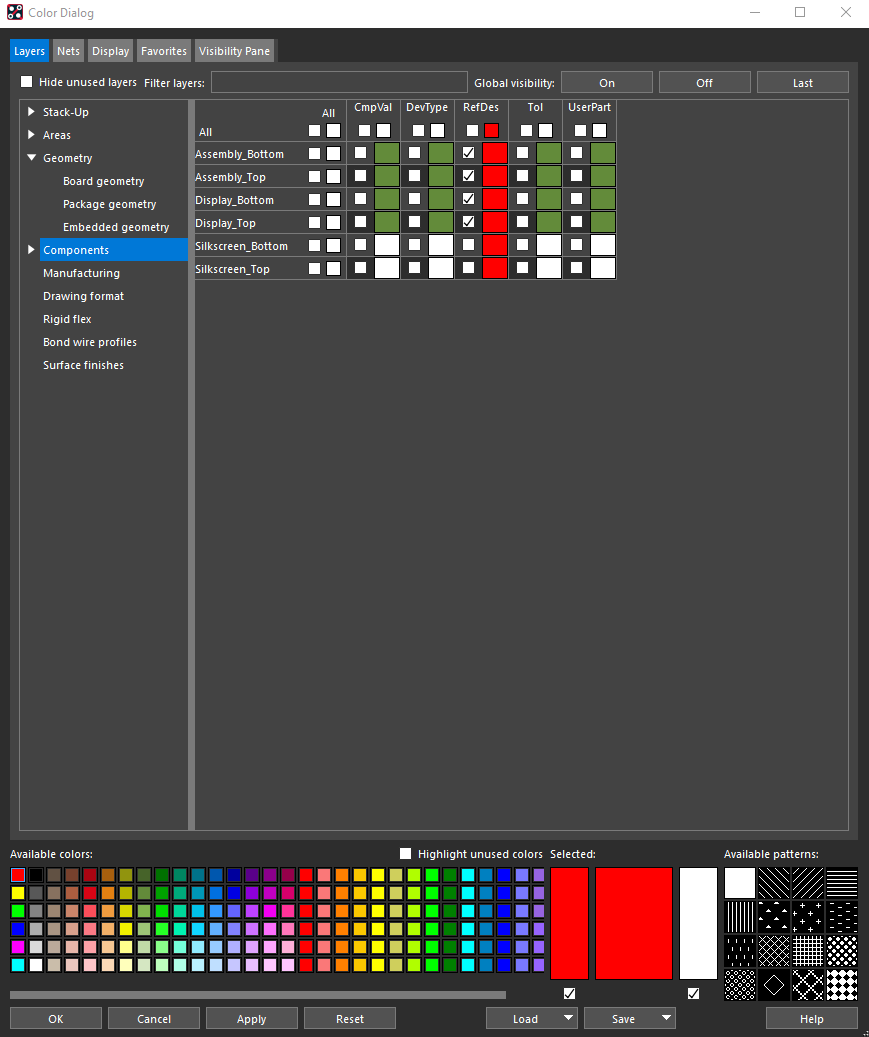
\includegraphics{AllegroImages/colorsComponents.png}}
\caption{Component Colors}
\label{img:componentColors}
\end{figure}

Again, to remove more bloat text navigate to the "Components" tab and uncheck all columns except the "RefDes" column. The RefDes column
will put a text identifier next to every component that is the same as in the schematic, making it easy to identify what is what.

\begin{figure}[H]
  \centering
  \scalebox{.45}{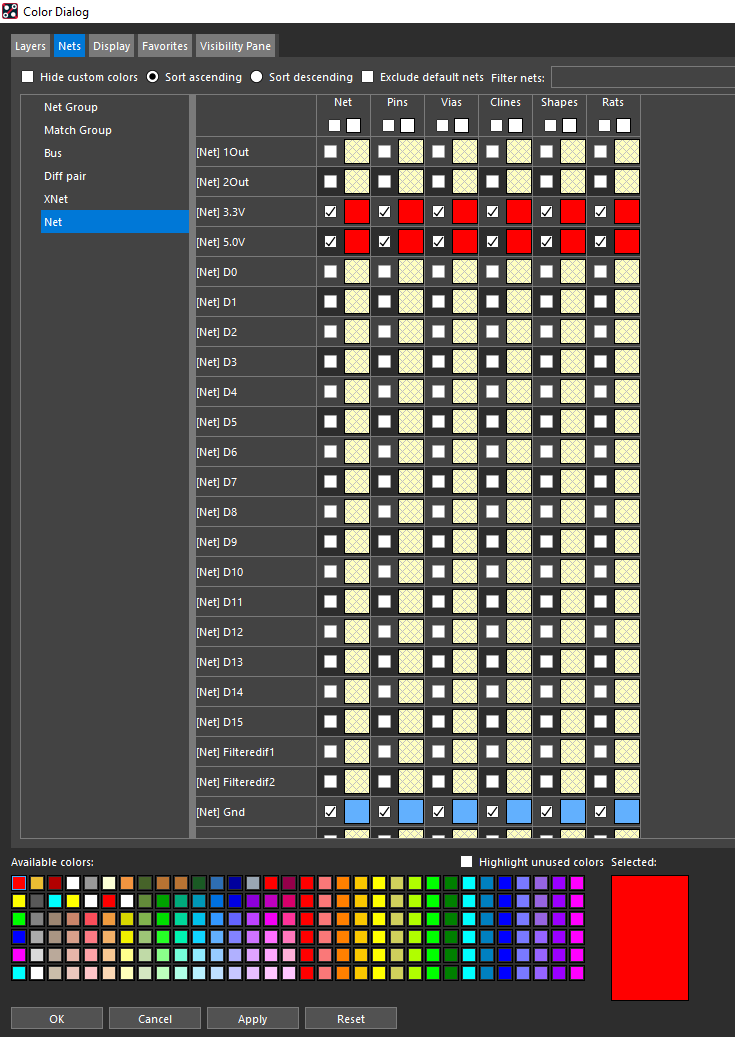
\includegraphics{AllegroImages/netsColors.png}}
\caption{Net Colors}
\label{img:netColors}
\end{figure}

At the top of the colors dialog you can select the nets tab as seen in Figure \ref{img:netColors}. When we draw our traces,
the traces by default will be colored what we selected in the stack-up 

\subsection*{Database Preparation}

\begin{figure}[H]
  \centering
  \scalebox{.45}{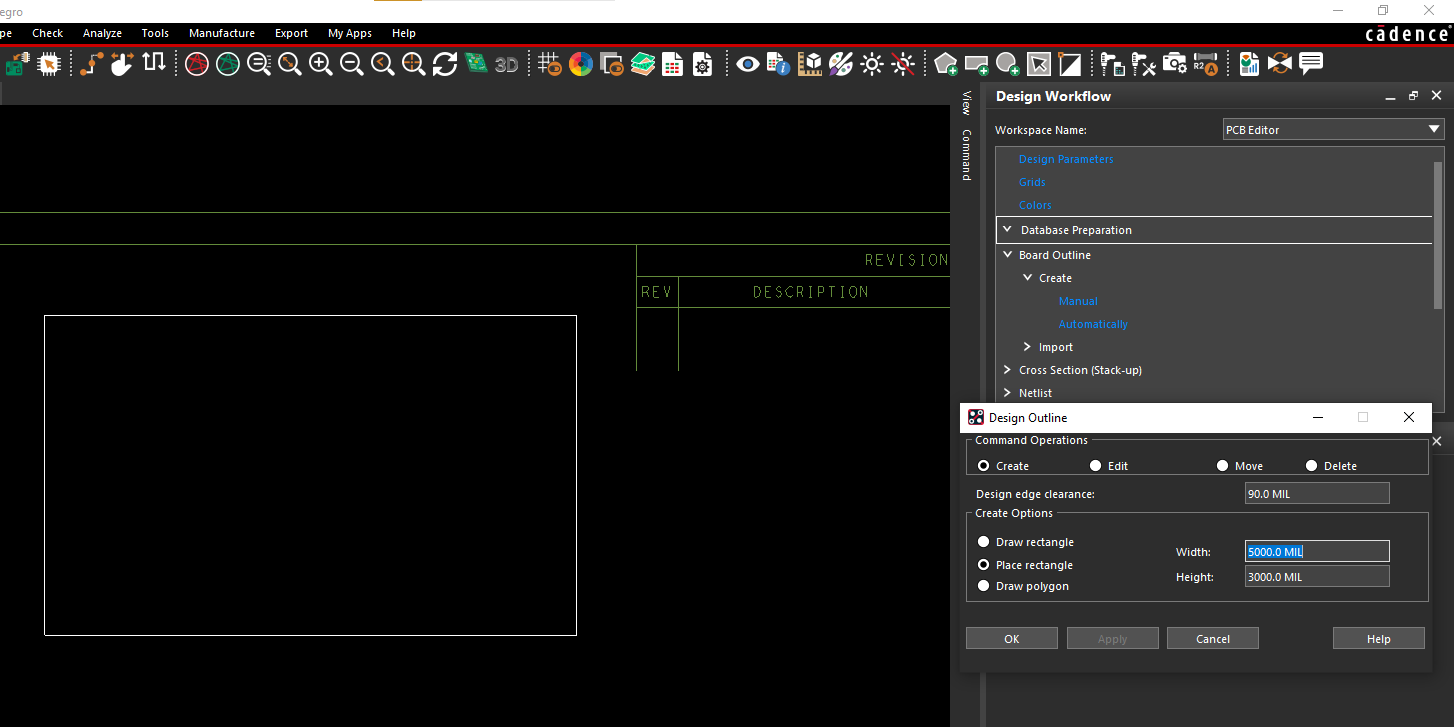
\includegraphics{AllegroImages/boardOutline.png}}
\caption{Board Outline}
\label{img:boardoutline}
\end{figure}

Now that our tool is setup, we can begin in our design. The first section in the Database Preparation is "Board Outline" which can be seen
in Figure \ref{img:boardoutline}. The board outline is for the designer to know the boundary of their future PCB.
Pick the "automatically" option under board outline to get the prompt in the figure. Click create in the prompt,
and then click "Place Rectangle". Now you can enter the design edge clearance, which will dictate how far from the edge of the board you can
place traces or components. Violating the clearance will pop up an error on your design for you to adjust accordingly. After entering your
design clearance, you can enter the length and width of your desired board and a white line will appear that you can move around with your cursor.
Then you can click for the final board and clearance outlines to be drawn.

